\let\negmedspace\undefined
\let\negthickspace\undefined
\documentclass[journal,12pt,onecolumn]{IEEEtran}
\usepackage{cite}
\usepackage{amsmath,amssymb,amsfonts,amsthm}
\usepackage{algorithmic}
\usepackage{graphicx}
\graphicspath{{./figs/}}
\usepackage{textcomp}
\usepackage{xcolor}
\usepackage{txfonts}
\usepackage{listings}
\usepackage{enumitem}
\usepackage{mathtools}
\usepackage{gensymb}
\usepackage{comment}
\usepackage{caption}
\usepackage[breaklinks=true]{hyperref}
\usepackage{tkz-euclide} 
\usepackage{listings}
\usepackage{gvv}                                        
%\def\inputGnumericTable{}                                 
\usepackage[latin1]{inputenc}     
\usepackage{xparse}
\usepackage{color}                                            
\usepackage{array}
\usepackage{longtable}                                       
\usepackage{calc}                                             
\usepackage{multirow}
\usepackage{multicol}
\usepackage{hhline}                                           
\usepackage{ifthen}                                           
\usepackage{lscape}
\usepackage{tabularx}
\usepackage{array}
\usepackage{float}
\newtheorem{theorem}{Theorem}[section]
\newtheorem{problem}{Problem}
\newtheorem{proposition}{Proposition}[section]
\newtheorem{lemma}{Lemma}[section]
\newtheorem{corollary}[theorem]{Corollary}
\newtheorem{example}{Example}[section]
\newtheorem{definition}[problem]{Definition}
\newcommand{\BEQA}{\begin{eqnarray}}
\newcommand{\EEQA}{\end{eqnarray}}
\newcommand{\define}{\stackrel{\triangle}{=}}
\theoremstyle{remark}
\newtheorem{rem}{Remark}

\begin{document}
\title{1.6.11}
\author{EE25BTECH11061 - Vankudoth Sainadh}
\maketitle
\renewcommand{\thefigure}{\theenumi}
\renewcommand{\thetable}{\theenumi}

\textbf{Question:} If the points $A(1,2)$, $O(0,0)$ and $C(a,b)$ are collinear, find the relation between $a$ and $b$.

\medskip
\textbf{Solution (Rank \& Row-Reduction Method).}

\textbf{Step 1: Write the points.}
\begin{align*}
\vec{A} &= \myvec{1\\[2pt]2}, &
\vec{O} &= \myvec{0\\[2pt]0}, &
\vec{C} &= \myvec{a\\[2pt]b}.
\end{align*}

\textbf{Step 2: Form difference vectors relative to $\vec{A}$.}
\begin{align*}
\vec{O}-\vec{A} &= \myvec{0\\0} - \myvec{1\\2} = \myvec{-1\\[2pt]-2},\\
\vec{C}-\vec{A} &= \myvec{a\\b} - \myvec{1\\2} = \myvec{a-1\\[2pt]b-2}.
\end{align*}

\textbf{Step 3: Build the matrix and state the rank condition for collinearity.}
\begin{align*}
M &= \big(\,\vec{O}-\vec{A}\;\; \vec{C}-\vec{A}\,\big)^{T}
   = \myvec{-1 & -2\\[4pt] a-1 & b-2},\\
\text{Collinearity} &\iff \operatorname{rank}(M)=1.
\end{align*}

\textbf{Step 4: Row elimination (make the $(2,1)$ entry zero).}
\begin{align*}
R_2 &\longrightarrow R_2 - \frac{a-1}{-1}\,R_1
\quad (\text{note: }-1\neq 0),\\[6pt]
\myvec{-1 & -2\\ a-1 & b-2}
&\longrightarrow
\myvec{-1 & -2\\ 0  & b-2a}.
\end{align*}

\textbf{Step 5: Rank condition.}
\begin{align*}
\operatorname{rank}(M)=1
\;\Longleftrightarrow\;
\text{second row is the zero row}
\;\Longleftrightarrow\;
b-2a=0.
\end{align*}

\textbf{Step 6: Final relation.}
\begin{align*}
\boxed{\,b=2a\,}.
\end{align*}

\newpage
\begin{figure}[h!]
\centering
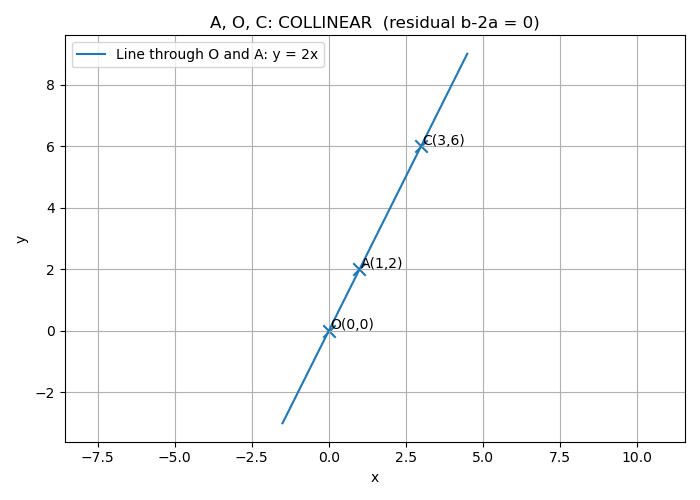
\includegraphics[width=0.7\columnwidth]{figs/Figure_1.png}
\caption{}
\label{}
\end{figure}

\end{document}
